\chapter{Configuring the TransistorTester}
\label{sec:config}
The complete software for the TransistorTester is available in source code.
The compilation of modules is controlled with a Makefile. The developement was done
at the Ubuntu Linux operating system with the GNU toolchain (gcc version 4.5.3).
It should be possible to use other Linux operating systems without problems.
To load the compiled data to the flash memory or
the EEprom memory, the tool avrdude (version 5.11svn) was taken by the Makefile, if you call ``make upload''.
 The program avrdude is available for Linux and Windows operating system.
The gnu C-compiler gcc is also taken by the AVR studio software
at the Windows operating system.
You can load the program data (.hex and .eep) also with other tools to the ATmega,
but only my Makefile version takes care to load the correct data to the choosed processor.
Avrdude loads only data to the ATmega if the Signature Bytes of the connected ATmega is
identical to the choosed one. 
If you alter the Makefile, all the software will be compiled new, if you call a ``make'' or
``make upload'' command. The software compiled for a ATmega8 does not run on a ATmega88.
The software compiled for a ATmega168 does not run on the ATmega88, even if the ATmega88 has enough flash memory! 
Be careful, if you don't use my Makefile.


The following options in the Makefile are avaiable to configure the software for your Tester.

\begin{description}
  \item[PARTNO] describes the target processor:\\
         m8 = ATmega8\\
         m48 or m48p = ATmega48\\
         m88 or m88p = ATmega88\\
         m168 or m168p = ATmega168\\
         m328 or m328p = ATmega328\\
    example:  PARTNO = m168
  \item[UI\_LANGUAGE] specifies the favored Language\\
    LANG\_ENGLISH, LANG\_GERMAN, LANG\_POLISH, LANG\_CZECH, LANG\_SLOVAK and LANG\_SLOVENE is currently avaiable \\
    example:  UI\_LANGUAGE = LANG\_ENGLISH
  \item[LCD\_CYRILLIC] is only needed for a LCD-display with cyrillic character set. The \(\mu\) and \(\Omega\) character
is not avaiable with the cyrillic character set.
If you specify this option, both characters are loaded to the LCD with software.\\
example: CFLAGS += -DLCD\_CYRILLIC
  \item[WITH\_SELFTEST] If you specify this Option, software will include a selftest function.
Selftest will be started, if you connect all three probes together and start measurement.\\
example: CFLAGS += -DWITH\_SELFTEST
  \item[R\_MESS] enables the resistor measurement. This option should allways be set.\\
example: CFLAGS += -DR\_MESS
  \item[C\_MESS] enables the capacity measurement. This option should allways be set.\\
example: CFLAGS += -DC\_MESS
  \item[CAP\_EMPTY\_LEVEL]  This option defines the voltage level for discharged capacitor (mV units).
You can set the level to higher value as 3mV, if the tester does not finish discharging of capacitors.
In this case the tester ends after longer time with the message ``Cell!''.\\
example: CFLAGS += -DCAP\_EMPTY\_LEVEL=3
  \item[WITH\_AUTO\_REF] specifies, that reference voltage is read to get the actual factor for capacity measuring of low capacity values (below \(50\mu F\)).\\
example:  CFLAGS += -DWITH\_AUTO\_REF
  \item[REF\_KORR] specifies an offset for readed reference voltage in mV units.
This can be used to adjust the capacity measurement in the WITH\_AUTO\_REF mode.\\
example:  CFLAGS += -DREF\_KORR=14
  \item[AUTOSCALE\_ADC] enables the automatic scale switchover of the ADC to either VCC or internal reference.
Internal reference gives a 2.56V scale for ATmega8 and a 1.1V scale for other processors.\\
example: CFLAGS += -DAUTOSCALE\_ADC
  \item[NO\_AREF\_CAP] tells your Software, that you have no Capacitor installed at pin AREF (pin 21).
This enables a shorter wait-time for the AUTOSCALE\_ADC scale switching of the ADC.
A 1nF capacitor was tested in this mode without detected errors.
Figure \ref{pic:aref1} and \ref{pic:aref5} show the switching time with a 1nF capacitor.
As you can see the switching from 5V to 1.1V is much slower than switching back to 5V. If you
have still installed the 100nF, switching time will be about factor 100 longer!\\
example: CFLAGS += -DNO\_AREF\_CAP
  \item[OP\_MHZ] tells your software at which Clock Frequency in MHz your Tester will operate.
The software is tested only for 1 MHz and 8Mhz. The 8MHz operation is recommended for better resolution of capacity measurement.\\
example: OP\_MHZ = 8
  \item[USE\_EEPROM] specifies if you wish to locate fix text and tables in EEprom Memory. Otherwise the flash memory is used.
Recommended is to use the EEprom (option set).\\
example: CFLAGS += -DUSE\_EEPROM
  \item[PULLUP\_DISABLE] specifies, that you don't need the internal pull-up resistors.
 You must have installed a external pull-up resistor at pin 13 (PD7) to VCC, if you use this option.
This option prevents a possible influence of pull-up resistors at the measuring ports (Port B and Port C).\\
example: CFLAGS += -DPULLUP\_DISABLE
  \item[ANZ\_MESS] this option specifies, how often an ADC value is read and accumulated.
Possible values for 5V Operation are 44, 22 and 11. The 44 gives best accuracy, but the longest measurement time.
One ADC measurement with 44~values takes about 4.7ms.\\
example: CFLAGS += -DANZ\_MESS=44
  \item[POWER\_OFF] This option enables the automatic power off function. If you don't specify this option,
 measurements are done in a loop infinitely  until power is disconnected with a ON/OFF switch.
If you have the tester without the power off transistors, you can deselect the option POWER\_OFF.
If you have NOT selected the POWER\_OFF option with the transistors installed,
you can stop measuring by holding the key several seconds after a result is displayed until the time out message is shown.
After releasing the key, the tester will be shut off by timeout.
You can also specify, after how many measurements without a founded part the tester will shut down.
The tester will also shut down the power after twice as much measurements are done in sequence without a
single failed part search. If you have forgotten to unconnect a test part, total discharging of battery is avoided. 
Specify the option with a form like CFLAGS += -DPOWER\_OFF=5 for a shut off after 5 consecutive measurements
without part found. Also 10~measurements with any founded part one after another will shut down.
Only if any sequence is interrupted by the other type, measurement continues.
The result of measurement stay on the display for 10~seconds for the single measurement, for the
multiple measurement version display time is reduced to 3~seconds (set in config.h).
The maximum value is 255 (CFLAGS += -DPOWER\_OFF=255).
  \item[BAT\_CHECK] enables the Battery Voltage Check. If you don't select this option, the version number of
software is output to the LCD instead.
This option is usefull for battery powered tester version to remember for the battery change.\\
example: CFLAGS += -DBAT\_CHECK
  \item[BAT\_OUT] enables Battery Voltage Output on LCD (if BAT\_CHECK is selected).
 If your 9V supply has a diode installed, use the BAT\_OUT=600 form to specify the threshold voltage (mV) of your diode
to adjust the output value.
Also the voltage loss of transistor T3 can be respected with this option.
 threshold level does not affect the voltage checking levels (BAT\_POOR).\\
examples: CFLAGS += -DBAT\_OUT=300  or CFLAGS += -DBAT\_OUT
  \item[BAT\_POOR] sets the poor level of battery voltage to the specified 100mV (1/10 Volt) value.
The warning level of battery voltage is always 1V higher than the specified poor level.
Setting the poor level to low values such as 5.4V is not recommended for rechargeable 9V batteries,
because this increase the risk of battery damage by the reason of the deep discharge!
If you use a rechargeable 9V Battery, it is recommended to use a Ready To Use type, because of the lower self-discharge.\\
example for low drop regulator (5.4V): CFLAGS += -DBAT\_POOR=54
example for 7805 type regulator (6.4V): CFLAGS += -DBAT\_POOR=64
  \item[PROGRAMMER] select your programmer type for avrdude interface program.
The correct selection of this option is needed, if you use the ``make upload'' or ``make fuses'' call
of this Makefile.
For further information please look to the manual pages of avrdude and online documentation~\cite{avrdude}.\\
example: PROGRAMMER=avrisp2
  \item[PORT] select the port where avrdude can reach your microcontroller (atmega).
and port if you will use avrdude
For further information please look to the manual pages of avrdude.\\
example: PORT=usb

\end{description}

\begin{figure}[H]
  \begin{subfigure}[b]{9cm}
    \centering
    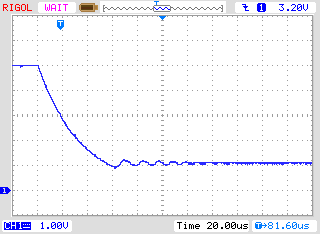
\includegraphics[width=9cm]{../PNG/AREF2_1V.png}
    \caption{from 5V to 1.1V }
    \label{pic:aref1}
  \end{subfigure}
  ~
  \begin{subfigure}[b]{9cm}
    \centering
    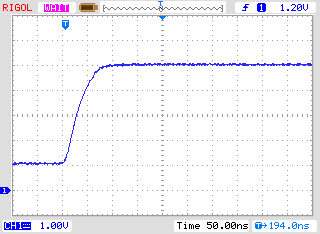
\includegraphics[width=9cm]{../PNG/AREF2VCC.png}
    \caption{from 1.1V to 5V}
    \label{pic:aref5}
  \end{subfigure}
  \caption{AREF switching with a \(1nF\) Capacitor}
\end{figure}


Additional parameters can be set in the files transistortester.h and config.h .
The file transistortester.h contains global variables and defines the port / pin constellation
and the resistor values used for measurement.
The file config.h specifies parameter for different processor types, wait times and the clock
frequency of the ADC. Normally there is no reason to change these values.
